\section{Iteration No 2: Performance Improvements}
\label{sec:iteration_no2}

In the previous section the prototype was successfully deployed and tested.
The next step is to move this from a \ac{MVP} to a more stable and performant environment,
this includes improving deployment and execution times,
as well as properly addressing previous workarounds.

\subsection{Milestones and Goals}

\begin{enumerate}
    \item \textbf{Deploy time:} As the image contains the entire Chapel compiler, its source code as wellas
          the Arkouda client library and its dependencies, the image is quite large. This slows down the deployment
          process, as the image needs to be transferred to the cluster and then unpacked. The goal is to reduce the
          size of the image to speed up the deployment process.
    \item \textbf{Container Runtime:} The current container \ac{CRI} is \textit{Containerd} which, while being
          lightweight, is not the fastest \ac{CRI} available. The goal is to switch to a faster \ac{CRI} more suited to
          \ac{HPC} workloads, such as \textit{Singularity}.
    \item \textbf{Investigating Arkouda Crash:} During the previous iteration, the Arkouda environment crashed
          when running the \textit{argsort} function on a string array. This was fixed by \gls{monkey patching} in the
          \textit{NumPy} implementation. The goal is to investigate the cause of the crash and fix it properly, to
          gain back the performance lost by using the \textit{NumPy} implementation.
    \item \textbf{Performance Testing:} In order to even quantify the performance in the first place,
          a way to measure the performance needs to be established. This will be done by running a set of benchmarks
          before and after the changes are made.
\end{enumerate}

\subsection{Implementation}

\subsubsection{Deploy time}

The time it takes a service from being requested and being available is crucial for the flexibility of a
Kubernetes cluster, as this determines how fast the cluster can adjust to changing workloads, increasing
demand or failures.  The current size of the image as reported by \textit{podman} is 3 GB, which is quite large,
for a simple client service. This is due to the fact that the e ntire Chapel project as well as all build tools are included in the image.
Having such a large image slows down the deployment process, as the image needs to be transferred and unpacked to the node.
One solution to this is prefetching the image on the nodes, is called \textit{image pre-pulling}.
Taking the time it takes to pull the image at an earlier time and storing a local copy on the node,
this way the image is already available when the service is requested.
This is feasible for small clusters with a low diversity of images, but the overhead of keeping local copies of
images locally, scales quadratically with the number of images and nodes, as each image needs to be stored on each node.
Therefore, we want to investigate by how much we can reduce the size of the image, to speed up the deployment process.

For this reason a script was written to measure the time it takes to deploy an image.
More about how this testing works can be found in the Performance Testing section of this iteration.

\begin{figure}[!ht]
    \vspace{0.8cm}
    \centering
    \scalebox{0.7}{
        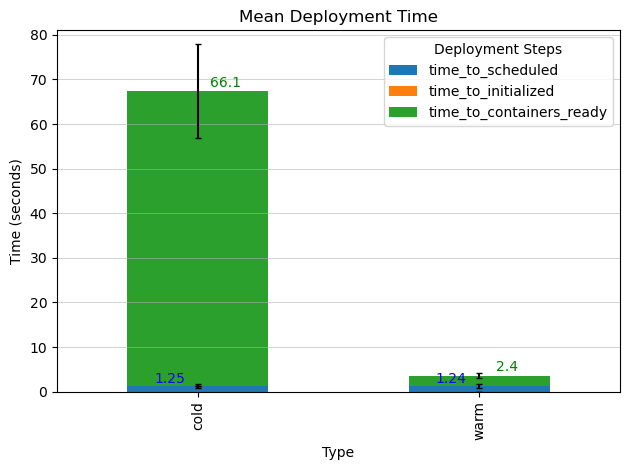
\includegraphics{./graphics/deployment-time-large-image.png}
    }
    \caption{Deployment time of a 2.86GB image\protect\footnotemark}
    \label{fig:deployment_time_large_image}
\end{figure}
\footnotetext{Data can be found in the project repo at \cite{joneckerthBachelorThesisProjecta}}

Figure \ref{fig:deployment_time_large_image} above shows the time the different steps of the deployment process take in seconds.
In blue is the time it takes from requesting the deployment of a service until Kubernetes assigns the pod to a node.
In the orange section we would see the time it takes the initialization containers of the pod to start.
The init-containers are needed to set up the namespace and network for the pod;
they pull and start the actual container image (see \Nameref{sec:containerization}).
However, as Kubernetes can only measure events with a resolution of seconds,
and these containers are ready in milliseconds, hey are too short to be measured reliably by Kubernetes.
Going from requested to ready in between the polling makes it seem like they are ready instantly.
The green section is the time it takes from the initialization containers being started to the whole pod
being able to accept requests. This includes the time it takes to pull the image from the registry, unpack it,
the start of the container and the time for the software inside the container to be ready to accept requests\footcite{kubernetes-docsPodLifecycle}.

With all else being equal we can clearly see the large difference between fetching the image from the registry,
and having the image already available on the node.
As container images are built out of \ac{COW} layers (see \Nameref{sec:docker}),
one can specifically target the layers which are the largest and try to reduce their size.
One thing to note is, that due to every command creating a new immutable layer,
one should try to chain commands together, to reduce the number of layers created.
So instead of creating a layer for the installation of a package, another layer for the usage
and a third layer for the removal of the package, one should chain these commands together in one layer to
result in a single layer containing only the artifact needed for the package.
The most effective method to reduce the size of an image besides, choosing smaller base images,
and being mindful of the layers created, is to use multi-stage builds.
This is a feature of the Dockerfile format that allows you to create multiple images from a single Dockerfile.
Its main use case is to build the project in one image and then copy the build artifacts to a second image.
This is useful as the first image can contain all the tools and dependencies needed to build the project,
while the second image can be a much leaner distribution, only copying the build artifacts from the first stage over,
reducing the overall size of the image significantly, while making the build process easier.

These practices were applied to our initial image, reducing the size from 2.86 GB down
to  710 MB, a reduction which is a largely due to the use of multi-stage builds,
replacing the Chapel image after the Chapel build was done. Additional size reduction
could be achieved by isolating the python modules after the Chapel build process and
moving them using a \ac{VENV} to the final image.

Overall the size reduction of the image had a significant impact on the deployment time as
can be seen in figure \ref{fig:deployment_time_small_image} below.,
reducing the median deployment time of a non-pre-pulled image from 63.47 to 19.7 seconds,
a reduction of 69\%, which is nice for a simple change in the Dockerfile.

\begin{figure}[!ht]
    \vspace{0.8cm}
    \centering
    \scalebox{0.7}{
        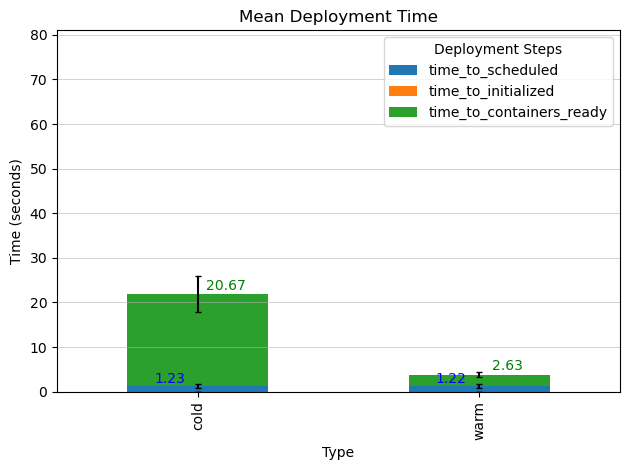
\includegraphics{./graphics/deployment-time-small-image.png}
    }
    \caption{Deployment time of a 710 MB image\protect\footnotemark}
    \label{fig:deployment_time_small_image}
\end{figure}

\footnotetext{Data can be found in the project repo at \cite{joneckerthBachelorThesisProject}}

But if we compare the difference the build makes on the prepulled image,
we can barely see any difference, both being around 2 seconds.
Being so close to a resolution of 1 second we can not see much of an effect.

As the images of the \ac{HPC} are taken from the Chapel and Arkouda projects,
they can also be given the same treatment, as the images are quite large as well.
While the Arkouda server and locale environment are even larger than the Jupyter image,
they are also much more complex, and rely on more than just the python bindings to work.
Multi-stage builds are especially important here since the tooling needed to compile
the chapel project alone already make up more than a gigabyte of the image.
It is also built on top of the original Chapel image, which is already quite large,
containing the precompiled Chapel binaries, saving the time of compiling Chapel during the build process.
But compiling both Chapel and Arkouda from source, using multi-stage builds,
and \ac{VENV}s to isolate the python modules, we were able to reduce the size of the image significantly.
The size of the Arkouda image was reduced from 3.88 GB to 1.08 GB, a reduction of 72\%
an effect which is even more important than the reduction of the Jupyter image,
as the Arkouda images will be running on each and every node in the cluster,
being scaled up and down as needed, making the flexibility of them quite important.


\subsubsection{Container Runtime}
\label{sec:container_runtime}

As can be seen from the diagrams above, the significant effect changing the size of the image has on the deployment time,
only effects the time it takes pulling and unpacking the image, but not the startup time or the time it takes for the software to be ready.
The setup time for a prepared container is mostly determined by the software inside the container as well as the overhead of container,
which is determined by the \ac{CRI} used.
WRewriting Jupyter notebook or a \ac{HPC} scale parallel processing framework like Chapel to be faster is certainly out of
scope for this thesis, however on the other hand changing the \ac{CRI} is a much more manageable task,
which will also might prove beneficial to later iterations as discussed in the \Nameref{suggested_architecture}.

Replacing the \ac{CRI} on a running Kubernetes cluster is akin to changing the engine of a car while it
is still running, as the \ac{CRI} is responsible for the runtime of the containers, and is responsible for
starting and stopping the containers, as well as managing the container's lifecycle.
Completely replacing an all-purpose \ac{CRI} like \textit{Containerd} with a
\ac{HPC} optimized \ac{CRI} like \textit{Singularity} might have unforeseen consequences.
Therefore, having both available on the same nodes, and utilizing whichever is more suited for the task at hand,
would be ideal.

Unfortunately, this step proved to be more difficult than anticipated,
as the \textit {Singularity} \ac{CRI} documentation claims to be able to run on a Kubernetes cluster,
which is not untrue;
But due to the singularity becoming a part of the open software foundation in 2015,
the project has been split into a community edition being maintained by volunteers,
and a completely rebranded version called \textit{Apptainer} which has moved away
from the \ac{HPC} space completely focusing now on subjects such as \textit{Sigstore} and Continuous Delivery.
The original version of \textit{Singularity} is still available on the \textit{Sylabs} website,
but has not been updated in the last 5 years, a fact which is not mentioned
when looking at the documentation\footcite{singularity-docsIntegratingKubernetesSingularity},
only visible when looking at the actual code of the project\footcite{singularity-repoSylabsSingularitycriSingularity}.
The version of \textit{Singularity} that is being maintained by the community, and more up to date,
is much smaller in scope and decided to focus their efforts to core projects,
abandoning the \ac{CRI} implementation\footcite{singularity-repoSylabsSingularitycriSingularity}.
While it technically still possible to run a cluster with \textit{Singularity} running as a \ac{CRI},
it is not possible  to do so for any version of Kubernetes beyond 1.26.
This is due to the fact that the \textit{Singularity} \ac{CRI} is based on the now deprecated version \textit{v1alpha2}
which was removed in version 1.26\footcite{kubernetes1.26releaseteamKubernetesV1262022}.


It is possible to run a \textit{Singularity} container without the \ac{CRI} on a Kubernetes cluster,
as it supports the \ac{OCI} standard, which means that one can convert a \textit{Singularity} image
to any other \ac{OCI} compliant image, and then run it on the generic \ac{CNI} of Kubernetes.
The features of \textit{Singularity} that made it originally so attractive for \ac{HPC} workloads,
such as its native support for \ac{GPU}s and \textit{Infiniband}
would need to be implemented the hard way, in Kubernetes itself, which then would defeat the purpose of using
a different \ac{CRI} in the first place.

\subsection{Investigating Arkouda Crash}

As we touched on in the previous iteration (\ref{testing_iteration_no1}) we had a problem with the Arkouda environment
crashing when a certain function is called on a string array. At that point in time, tracking down the error
proved time-consuming, and once enough information was gathered a workaround was found by \gls{monkey patching}
the function to use the \textit{NumPy} implementation instead(which can be found in the project repo\footcite{joneckerthBachelorThesisProjectb}),
while leaving the proper fix for the next iteration, as the primary goal was to get the system up and running.
After further investigation the hypothesis was that the error was not actually a bug in the code,
but a mismatch in the communication protocol between the Jupyter server and the Arkouda server.
While both were using the same version of the Arkouda library the Arkouda was originally
build when the system was set up during the "Pachykouda" project; the Jupyter server being build
during the first iteration of this project, there might have been some changes within the containers
since then.

As we have been relying on these containers provided by the Chapel and Arkouda projects,
we have little control over the versions and the variables used to compile the binaries.
Additionally, these images are quite large, slowing down the deployment as discussed in the first iteration.
To reduce the size of the images and to gain more control over the environment,
the images were rebuilt from scratch.
So a common base image was created, containing all the necessary files and binaries needed for the client, server and locale images.
From this base image, the corresponding images were created,
having an identical common environment but including only the necessary files
for the specific image to be created.
Thereby ensuring that the environment is the same for all images and have
the same version of the binaries and libraries at heart.

After the images were successfully brought to a state were they could be used as
a drop-in replacement for the original images, the client was tested again, and the error was gone.



\subsection{Performance Testing}
\label{sec:performance_testing}

Originally it was planned to test both the effect of the image size on the deployment time,
as well as the effect of the \ac{CRI} on the startup time and the execution time of the software.
Due to the fact that \textit{Singularity} only supports \ac{OCI} based execution on kubernetes,
there would be no relevant difference as both get converted into the same container format\footcite{opencontainerinitiativeImagespecSpecMd2024},
making the effort of converting the compute nodes to \textit{Singularity} inefficient in
the context of this project.

But testing the startup time was still possible and with the conversion of the Arkouda images and the
reduction of the size of the Jupyter image, having a good sense of how quickly the system is able to respond
to changes in the workload is still important.
The testing was done by utilizing Kubernetes "Pod Conditions" which are a set of states a pod
transitions through in its lifecycle, which can be used to monitor the state of the pod\footcite{kubernetes-docsPodLifecycle}.
Being able to query this information with the Kubernetes API, we can measure the time it takes for a pod to go from
start of the request to the pod being scheduled on a node, the time it takes for the pod to be initialized and the time it takes for the pod to be ready to accept requests.

So in order to compare hot and cold starts, it was needed to make sure that during the first run,
all of the images were not pre-pulled, and during the second run, all the images were pre-pulled,
the former needing to be wiped from the corresponding nodes each time.
The results of the testing can be seen in the diagrams above, and show a significant difference between the two,
with the pre-pulled images being ready in a fraction of the time of the non pre-pulled images.
The tests were done with a sample size of 400 with the images being deployed on the whole cluster,
and the results were then aggregated to show the median time it takes for the images to be ready.
The code\footcite{joneckerthBachelorThesisProjecte}, the notebook of the analysis\footcite{joneckerthBachelorThesisProjectd} and the raw data\footcite{joneckerthBachelorThesisProjectc} can be found in the project repo.


But as we are planning to compare the performance improvements of future iterations, it is important to
establish a baseline anyhow, for this reason a testing environment was set up and benchmarks were run on the cluster.
In order to do this, the Jupyter client was modified to run the micro benchmarks provided by the Arkouda project\footcite{arkouda-repoArkoudaRepoBenchmarks}.
The micro benchmarks test the performance of each of the major functions, such as \textit{argsort}, \textit{sum} and \textit{aggregate},
on all the supported data types. Getting a very fine-grained view of the performance of the Arkouda environment,
in each and every aspect.
As the cluster has four nodes which are theoretically \ac{IB} capable,
and will be enabled in the next iteration,
the benchmarks were limited to four nodes as well in order to have a fair comparison.
The tests were run with a problem size from $10^6$ to $10^{11}$ items per array,
in order to show how the performance behaves with increasing problem sizes.
% Additionally a comparison with the \textit{NumPy} implementation was done, 
% to show the advantages and disadvantages of a distributed array implementation, 
% in contrast to a classical single node implementation.

\begin{figure}[!ht]
    \vspace{0.8cm}
    \centering
    \scalebox{0.55}{
        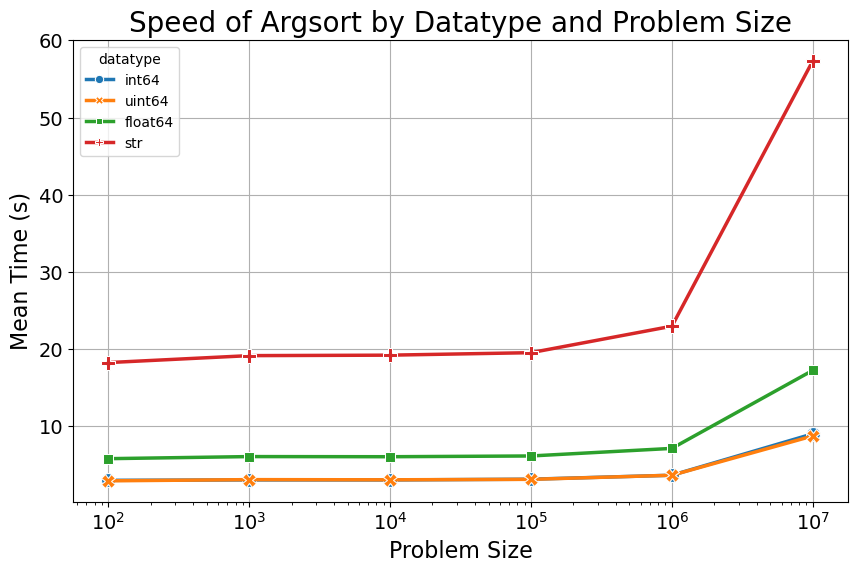
\includegraphics{./graphics/argsort.png}
    }
    \caption{Argosort by Problem Size}
    \label{fig:argsort}
\end{figure}
\footnotetext{Data available at: \cite{joneckerthBachelorThesisProjectf}}

The figure \ref{fig:argsort} above shows the how the performance of a tightly
coupled problem such as the \gls{argsort} function.
Here it can be seen how the time to solve the problem starts to increase exponentially,
corresponding to the problem size increasing by orders of magnitude for each test.

Another interesting aspect is the performance of the different data types,
as sorting a string array of the same length takes much longer than any other data type.
This is due to the variable length of strings in Arkouda, making the addressing
of the elements by index much more computationally expensive\footcite{arkouda-repoStringsArkoudaArkouda}

While \gls{argsort} implementing the sorting algorithm \textit{least-significant-digit radix sort}
demonstrates one of the worst cases for the performance an distributed system,
as it is a tightly coupled problem with a complexity of $O(w \cdot n)$,
were $w$ is the number of bits in the key and $n$ is the number of elements in the array.
The \textit{aggregate} function, shown in the diagram \ref{fig:agg_speed_by_datatype} below,
shows a much more diverse set of problems and how the performance of the system behaves with them.


\begin{figure}[!ht]
    \vspace{0.8cm}
    \centering
    \scalebox{0.55}{
        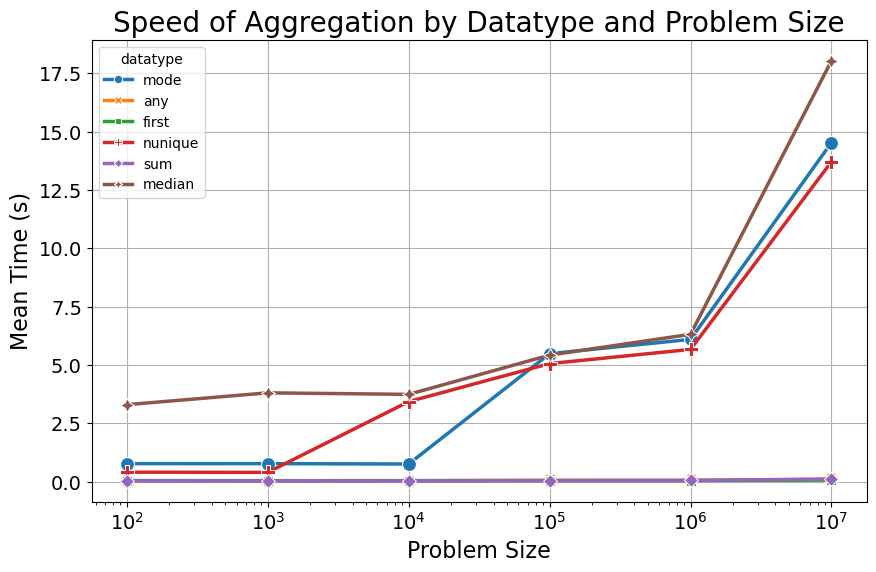
\includegraphics{./graphics/agg_speed_by_datatype.png}
    }
    \caption{Aggregated Speed by Data Type}
    \label{fig:agg_speed_by_datatype}
\end{figure}
\footnotetext{Data available at: \cite{joneckerthBachelorThesisProjectf}}

The figure \ref{fig:agg_speed_by_datatype} above shows clearly the wide gab in performance between
\textit{embarrassingly parallel} problems like \textit{sum}, \textit{any} or \text{first},
which are being split up into smaller problems and can be solved independently on each of the nodes,
without the need for any communication between them.
While less computationally expensive than \gls{argsort},
functions such as \textit{median} or \textit{mort} become time expensive,
as they can not be split up into smaller problems as easily.

So far the performance of the system has only been measured by the time it takes to solve
a problem of a certain length, but as the size of the elements themselves are not created equal,
or might even vary such as in the case of strings one should also take into account the actual
amount of data being processed.

Diagram \ref{fig:operation_data_transfer} is especially interesting as it shows the
clusters most extreme conditions. On one side the functions with the highest processing
rate and then the three functions with the slowest rate of processing.

\begin{figure}[!ht]
    \vspace{0.8cm}
    \centering
    \scalebox{0.6}{
        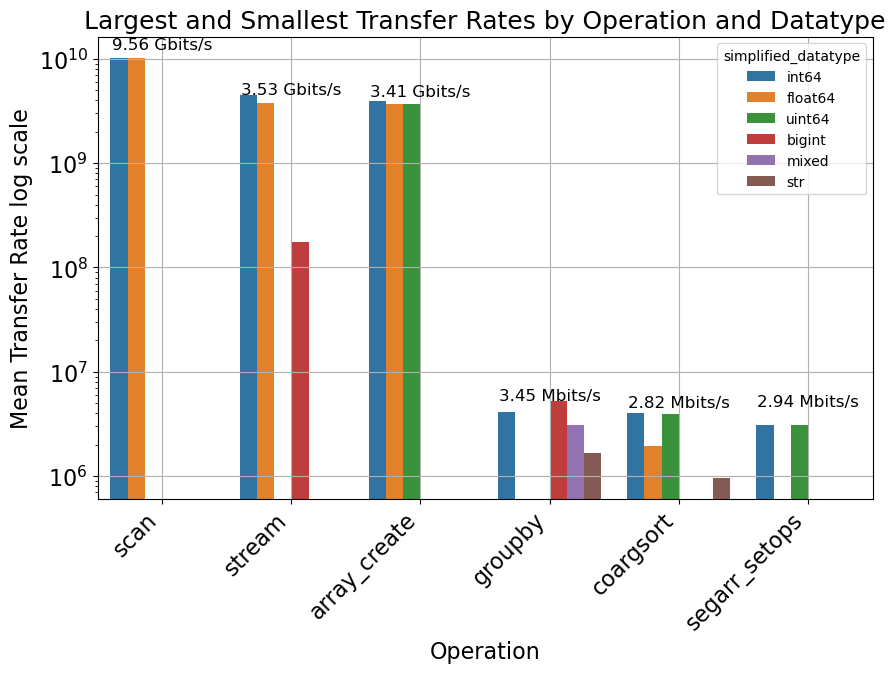
\includegraphics{./graphics/operation-data-transfer.png}
    }
    \caption{Operation Data Transfer}
    \label{fig:operation_data_transfer}
\end{figure}
\footnotetext{Data available at: \cite{joneckerthBachelorThesisProjectf}}

The speed of scanning the distributed array is essentially only limited by the speed of the underlying network,
as the data can be read in parallel from all nodes, and then aggregated on the client.
While the \textit{scan} function is very close the theoretical ideal of the network speed,
showing that the overhead of the whole network stack can be as low as 4.4\% under certain conditions;
The streaming function is not too far from the ideal processing speed of 30\%
of the network speed.
As the streaming function sends the \textit{axpy} operation to all nodes,
calculating $\displaystyle \boldsymbol {y} \leftarrow \alpha \boldsymbol {x}+ \boldsymbol {y}$.
Adding two arrays together while multiplying one of them by a scalar, this is a very simple and fast operation,
as each of the nodes can calculate the operation independently and then send the result back to the client.
The only delay being the time it takes to send the two arrays and receive the resulting array back.

The three arkouda functions which take the longest to process the data are
\textit{coargsort}, \textit{groupby} and \textit{segarr\_setopps}.
While \textit{groupby} directly calls the \textit{argsort} function and then performs
additional aggregations, \textit{coargsort} provides an index array just like \textit{argsort},
but instead of ordering it numerically it orders it by the order of another array.
As these functions just as \textit{argsort} are tightly coupled problems,
and rely on a lot of communication between the nodes, they are the slowest functions in the benchmark.
But the outlier in this case is the \textit{segarr\_setopps} function, which is a set operation on segmented arrays.
\textit{Segarr\_setopps} is even slower than complex sorting algorithm,
which seems counterintuitive at first, but the reason for this is that the function
has not been implemented for the distributed array yet \footcite{arkouda-docsSegArraysArkoudaArkouda},
and is being executed on the client negating the benefits of the distributed array implementation.

\subsection{Evaluation of Results}

The goal if this iteration was to move the \ac{MVP} to a more stable and performant environment,
reducing load times, fixing bugs and improving compute performance.
From this the need for a way to measure the performance in the first place was established.

The first goal, reducing the deploy-time by optimizing the image size of all parts of the system was
a complete success, with reductions in the size of the images around 70\% and the time to
deploy reduced significantly in the case of a non pre-pulled image.
While the original suggestion only intended to extend the images depending on our needs (see \Nameref{sec:container_image}),
during the prototyping phase the potential of large improvements were discovered,
and the decision was made to rebuild the images from scratch.

The second major goal, replacing the \ac{CRI} with \textit{Singularity} was not accomplished,
and the decision was made to not pursue this further,
as this would require updating a \ac{CRI} implementation which has been unsupported for the last 5 years.
While the performance increase would have had an impact on the container overhead,
a more significant impact would have been the native support for \textit{Infiniband} and \ac{GPU}s,
the former being especially important for \ac{HPC} workloads (see \ref{sec:networking_interconnects})
in but even more so with the current \ac{GASNet} implementation of Arkouda (see \ref{sec:gasnet}).
This gap in potential will be addressed again in the next iteration.

During the effort to rewrite the container images from scratch, the communication error was fixed,
and the Arkouda environment was running without any issues, passing all the unit tests and benchmarks.
The current theory being, that the issue was most likely due to a mismatch in the communication protocol,
between the jupyter server and the Arkouda server, which was fixed standardizing the versions across all images.

The last goal, establishing a baseline for the performance of the system was originally intended to be the basis
for the comparison between the \ac{CRI}s, but even though this was not possible, the benchmarks were still run,
in order to have a baseline for the performance of the system.

\subsection{Conclusion}

While some of the goals were successfully accomplished,
the goal of replacing the \ac{CRI} with \textit{Singularity} was not.
The performance of the image distribution was improved significantly,
and a baseline for the performance of the system was established.
The Arkouda environment was fixed and is now running without any issues.


\pagebreak